%\newpage
\section{Měření polovodičů}
Nejdříve má být u součástky zkoumán průběh proudu, s odpojeným ovládacím pinem (TP3),
(nazývaný také TriState pin). Ovládací pin je například (gate) nebo báze testované součástky.
Jeden testovací pin bude zvolen za kladnou stranu součástky a připojen přímo k VCC.
Jiný pin je pak považován za negativní stranu součástky.
Negativní strana bude připojena přes \(680\Omega\) odpor k GND.
U tranzistorů řízených polem je stav tranzistoru závislý na napájecím napětí.
(TP3) je nejprve pomocí \(680\Omega\) odporu připojen  k GND na \(5ms\) a zároveň změřeno napětí na negativní straně.\\Poté je TriState pin  přepnutý na vstup mcu (vysoká impedance) napětí opět změřeno.
Následovně je předpokládaný (gate) na \(5ms\) přes \(680\Omega\) odpor  přepnutý na VCC a napětí bude měřeno ještě jednou.
Pokud je měřené napětí nyní nižší než u prvního měření, bude tento stav přijat jako správný.
Nyní bude napětí s bezproudovým (TP3) ještě jednou změřeno.
Pokud je napětí záporného pinu s udržovanou úrovní větší než \(115mV\), tato úroveň není \(100mV\) nižší než úroveň s aktuálním (TP3), je předpokládán polovodič typu NPN minor chudý.
Pro bipolární tranzistory s vysokým zbytkovým proudem je zbytkový proud kolektoru 
v bázi mnohem vyšší.
Kontrolou obou úrovní se falešné detekci germaniových NPN tranzistorů s vyšším zbytkovým proudem kolektoru,
jako zchudlý typ N JFET tranzistorů, vyhneme.
Pak jsou provedeny další testy k rozlišení N-kanál JFET nebo D-MOSFET a P-kanál JFET nebo P-MOSFET.
Verze MOSFET mohou být detekovány nedostatkem řídícího proudu v každém stavu na (TP3).
Aby bylo možné měřit parametry typu N minor, je měřeno napětí na \(680\Omega\) odporu
na zdrojovém source pinu. Jak je znázorněno na obrázku \ref{fig:JFETcd}
Toto měření je místo obvyklého měření proudu na gate napětí na potenciálu zdroje uděláno,
kvůli relativně vysokému \(680\Omega\) odporu.
Tak by v mnoha případech charakteristický proud \(I_\mathrm{DSS}\) FET by nebyl dosažen.

\begin{figure}[H]
\centering
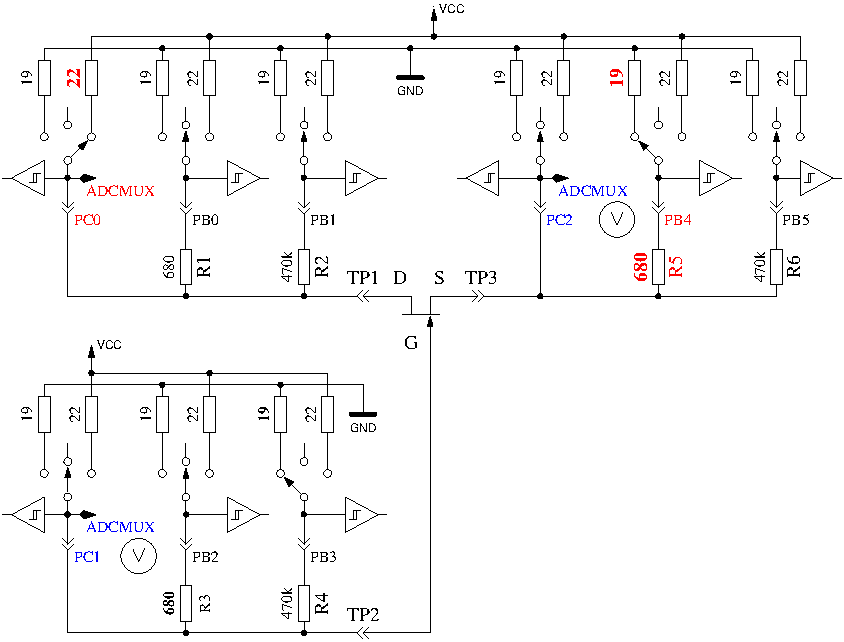
\includegraphics[width=.8\textwidth]{../FIG/JFETcd.pdf}
\caption{Měření Gate-Source-napětí a Source-proudu N-JFET-tranzistoru}
\label{fig:JFETcd}
\end{figure}

Pokud součástka nemá proud mezi kladným vývodem a záporným vývodem bez signálu
na (TP3) pinu jsou další testy popsány v další podkapitole \ref{sec:pnp}.
Pokud je zjištěn proud, jsou další testy popsány v podkapitole diody \ref{sec:diode}.

\subsection{Měření PNP tranzistoru nebo P-kanálu MOSFET}
\label{sec:pnp}
Za prvé je měřen aktuální faktor zesílení hFE v okruhu kolektoru (emitor následovník) pro předpokládaný
PNP tranzistor.
Situace měření je zobrazena na obrázku \ref{fig:pnpcc}.
Leží-li naměřené napětí báze (\(UB\)) přes \(9mV\) s \(680\Omega\) odporem,
bude aktuální zesílení hFE vypočítán pomocí \(hFE = \frac{UE-UB}{UB}\).
Napětí \(UE\) je rozdíl napětí emitoru k VCC. Rozdíl mezi \(22\Omega\) a \(19\Omega\) odporem se zanedbává.
\\Když leží \(UB\) napětí pod \(10mV\), bude měření provedeno s \(470k\Omega\) odporem v bázi.
V tomto případě bude vytvořen faktor zesílení proudu s \(hFE = \frac{UE \cdot 470000}{UB \cdot (680+22)}\).

\begin{figure}[H]
\centering
 \begin{overpic}[width=1.\textwidth]{../FIG/PNPcc.pdf}
  \color{black}
  \put(55,20){\makebox(0,0)[lb]{\textcolor{green}{Zeleně} označený stav nastane,}}  
  \put(55,17){\makebox(0,0)[lb]{když napětí na PC1 klesne  \textless~ 10mV!}}      
 \end{overpic}
\caption{+ měření PNP tranzistoru v kolektorovém obvodu}
\label{fig:pnpcc}
\end{figure}

Dále jsou testy pro předpokládaný PNP tranzistor v zapojení emitorový sledovač v obvodu emitoru.
Kladná strana je nyní připojena přímo k VCC, \(680\Omega\) odpor na záporném konci je připojen k GND,
jak je znázorněno na obrázku \ref{fig:pnpce}.
Pokud má záporná strana součástky napětí větší než \(3,4V\)  při použití \(680\Omega\) odporu na
bázi spojenou s GND, musí se jednat o PNP trazistor nebo o P-Kanal-FET.
To lze snadno rozlišit kontrolou napětí báze: pokud je větší než \(0,97V\), musí to být PNP.
Pro měření aktuálního faktoru zesílení bude namísto \(680\Omega\) odporu použitý \(470k\Omega\) jako odpor báze.
Aktuální zesílení se vypočítá pomocí \(hFE = \frac{(UC-UC0) \cdot 470000}{UB \cdot (680+19)}\).
Napětí UC0 je napětí na kolektorovém odporu bez proudu báze.
Vyšší faktor proudu je považován za správný, pro tento či onen zjištěný v kolektorovém obvodu.
Hodnoty zjištěné pro PNP tranzistor jsou platné pouze po provedení druhé sady měření.
Aby nedošlo k tomu, že by byl PNP tranzistor v inverzním obvodu, kdy je kolektor a emitor opačně, špatně detektován, bude jako správné měření použito to s vyšší hodnotou proudu.
Pokud je báze napětí menší než \(0,97V\), musí to být P-E-MOS.
V tomto případě je spínací napětí G řídící elektrody určeno tak, že je napětí na Gate s \(470k\Omega\) odporem pomalu měněno nahoru a dolů, dokud proud tekoucí přes vývod drain nevypne a potom je napětí na Gate měřeno.

\begin{figure}[H]
\centering
 \begin{overpic}[width=1.\textwidth]{../FIG/PNPce.pdf}
  \color{black}
  \put(55,21){\makebox(0,0)[lb]{Černý stav je používán při testu!}}  
  \put(55,17){\makebox(0,0)[lb]{\textcolor{green}{Zelený} stav se používá při}} 
  \put(55,13){\makebox(0,0)[lb]{proudovém zesílení faktoru hFE!}}      
 \end{overpic}
\caption{Testování a měření hFE PNP tranzistoru v emitorovém okruhu }
\label{fig:pnpce}
\end{figure}

\subsection{Měření NPN tranzistoru nebo N-kanálového MOSFETu}
Měření tranzistoru NPN začíná stejným způsobem jako měření PNP tranzistoru, jmenovitě
s měřením zesílení zesílení v kolektorovém obvodu.
První měření se provádí pomocí na VCC spojeným \(680\Omega\) bázovým odporem.
Pokud je napětí na bázovém odporu příliš malé, bude zde použitý \(470k\Omega\) odpor.
Měření pak pokračuje v emitorovém obvodu, jak je znázorněno na obrázku \ref{fig:npnce}.
\begin{figure}[H]
\centering
 \begin{overpic}[width=1.\textwidth]{../FIG/NPNce.pdf}
  \color{black}
  \put(55,23){\makebox(0,0)[lb]{Černý stav je používán při testu!}}  
  \put(55,19){\makebox(0,0)[lb]{\textcolor{green}{Zelený} stav se používá při}} 
  \put(55,15){\makebox(0,0)[lb]{proudovém zesílení faktoru hFE!}}      
 \end{overpic}
\caption{Testování a měření HFE tranzistoru NPN v emitorovém obvodu}
\label{fig:npnce}
\end{figure}
Pokud napětí na kolektoru je pod \(1,6V\) zatímco \(680\Omega\) je základní odpor
na VCC připojen, musí to být NPN, N-Kanal MOSFET nebo tyristor (TRIAC).
Dva jednoduché testy mohou detekovat tyristor nebo TRIAC.
Je-li Gate pin po dobu \(10ms\) připojen k GND a pak odpojen, měl by zůstat tyristor nebo triac sepnut.
Pokud se nyní anodový odpor krátce přepne na GND a poté se vrátí zpět na VCC,
neměl by tyristor znovu sepnout. Zůstane bez proudu.
Mějte na paměti, že lze testovat pouze tyristory s nízkým výkonem, protože spínací proud
testeru může dosáhnout pouze \(6mA\).
Pokud oba testy tyristor potvrdí, jsou prováděny další testy s obrácenou polaritou,
k vyloučení nebo potvrzení že se může jednat o TRIAC.
Pokud nebyl potvrzen žádný tyristor ani TRIAC, může to být NPN nebo N-kanálový E-MOSFET.
Napětí báze NPN tranzistoru se blíží napětí emitoru, čímž lze tento typ bezpečně rozpoznat.
Aktuální faktor zesílení v emitorovém okruhu je 
\(hFE = \frac{(VCC-UC-UC0)\cdot 470000}{(VCC-UB)\cdot (680+22)}\).
Pokud napětí na bázi ukazuje, že teče jen malý nebo žádný proud, jedná se zde o N-kanál E-MOS MOSFET.
V tomto případě je prahové napětí měřeno pomalým vzrůstem Gate napětí přes \(470k\Omega\) odpor střídavým připojením na VCC a GND a čeká až digitální signál na vstupu G sepne proud na Drain, aby v tom okamžiku bylo přečteno Gate napětí.
Měření se opakuje jedenáctkrát, jak je znázorněno na obrázku~\ref{fig:eleven}, a výsledky budou sčítány.
Vypočtená suma je násobena čtyřmi a pak dělena devíti, aby bylo dosaženo rozlišení v mV.

\begin{figure}[H]
\centering
\includegraphics[width=.8\textwidth]{../PNG/IRFU120gate.png}
\caption{Měření prahového napětí u N-kanálového MOSFETu}
\label{fig:eleven}
\end{figure}

\subsection{Zjednodušený proces identifikace tranzistorů}

\begin{figure}[H]
\centering
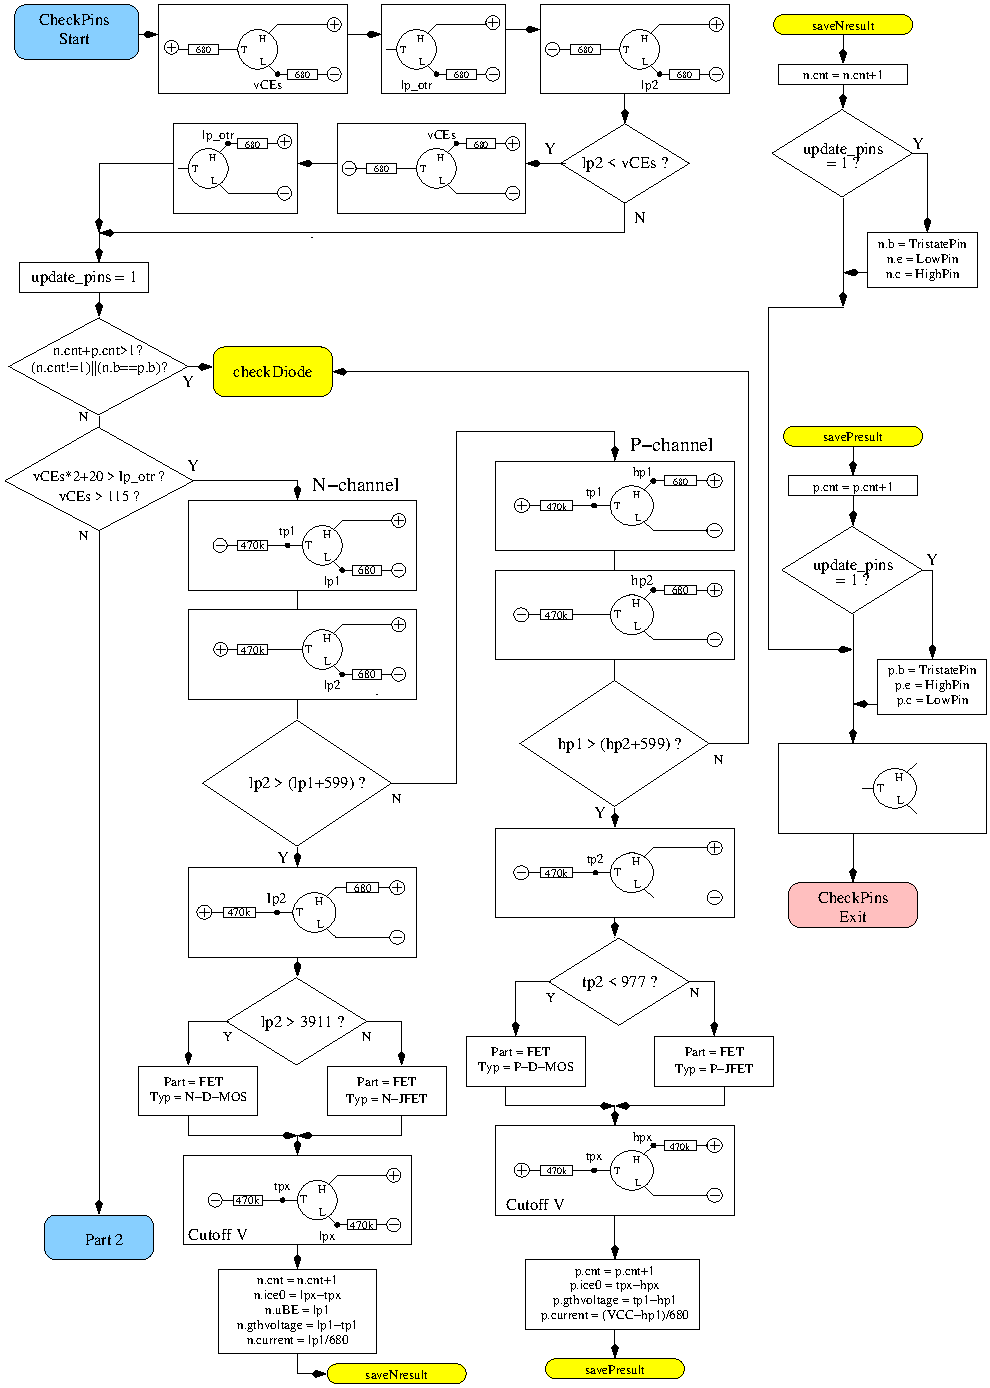
\includegraphics[width=.8\textwidth]{../FIG/CheckSemi1.pdf}
\caption{Program testování tranzistorů část 1, JFET a D-MOS}
\label{fig:ChkSemi1}
\end{figure}

\begin{figure}[H]
\centering
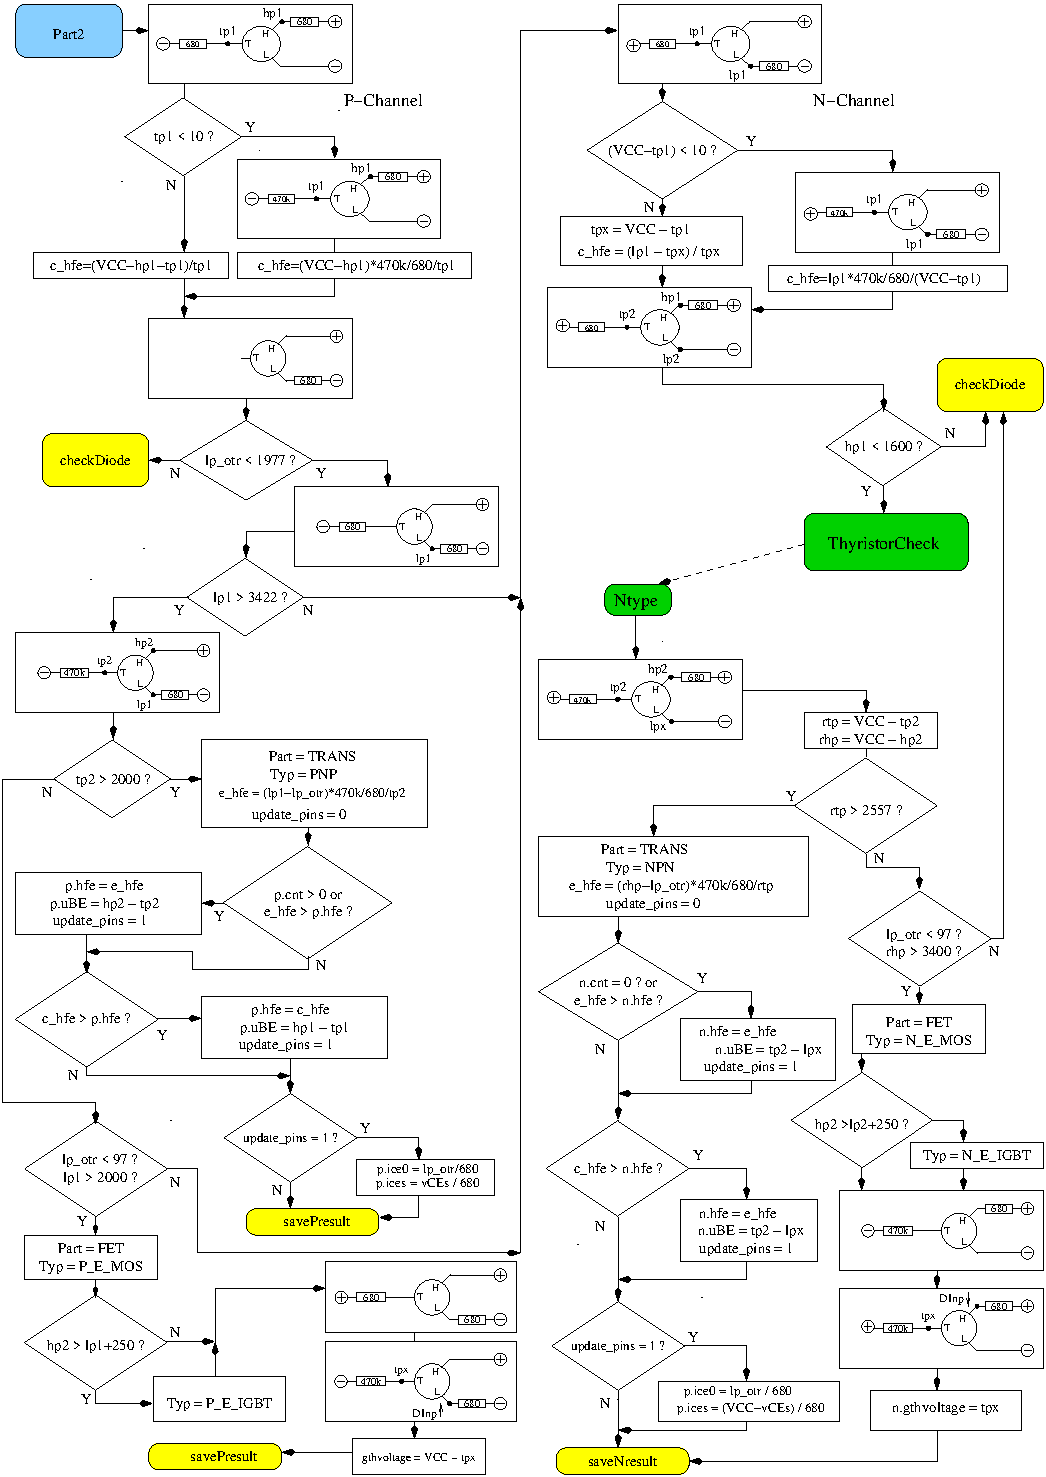
\includegraphics[width=.8\textwidth]{../FIG/CheckSemi2.pdf}
\caption{Program pro testování tranzistorů část 2, BJT a E-MOS}
\label{fig:ChkSemi2}
\end{figure}

\begin{figure}[H]
\centering
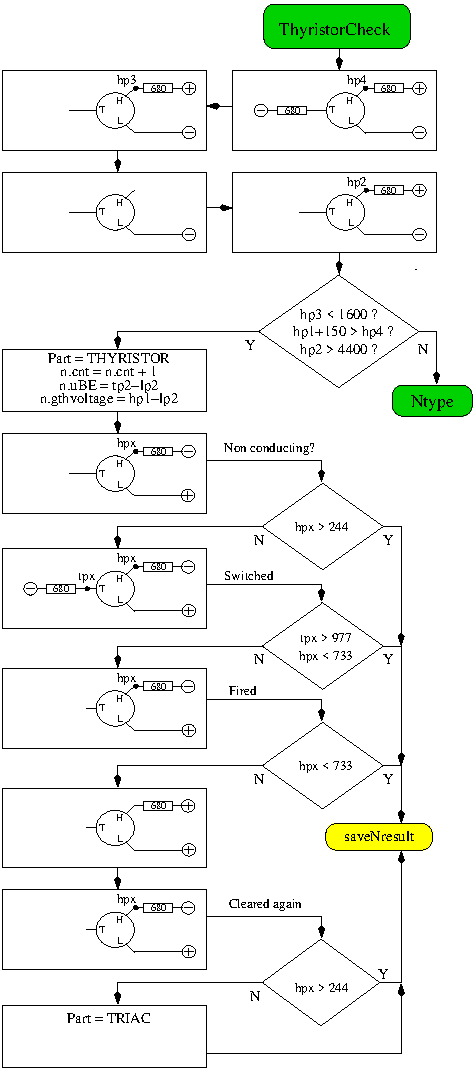
\includegraphics[width=.8\textwidth]{../FIG/CheckSemi3.pdf}
\caption{Program testování tranzistorů část 3, tyristor a triak}
\label{fig:ChkSemi3}
\end{figure}

\subsection{Měření diod}
\label{sec:diode}
Pokud byl v předběžných testech zjištěn proud, je součástka testována na chování diod.
Předpětí s \(680\Omega\) odporem musí být mezi \(0,15V\) a \(4,64V\).
Přední napětí s \(680\Omega\) odporem musí překročit 1,125 násobek dopředného napětí
s \(470k\Omega\) odporem a šestnáctinásobek dopředného napětí s \(470k\Omega\) odporem
větší než přední napětí s \(680\Omega\) odporem.
Navíc nesmí následné opětovné měření s \(470k\Omega\) odporem vydat vyšší napětí
než měření s \(680\Omega\) odporem.\\
Pak se dá předpokládat, že zařízení s tímto chováním je vždy dioda.
Detekce chování diody nedostatkem proudu v opačném směru není u antiparalelních diod možné.
Pro jednu diodu je přidán zpětný proud diody měřený u \(5V\) s \(470k\Omega\) odporem.
Rozlišení je asi \(2nA\). Pro větší zbytkové proudy než \(5,3\mu A\)
(napětí při odporu větší než \(2,5V\)) bude měřeno s \(680\Omega\) odporem.
Pak je rozlišení pouze \(1\mu A\).
Kromě toho se provádí měření kapacity diody v opačném směru. 

\subsection{Výsledky různých měření}
Následující tři tabulky zobrazují výsledky měření různých komponentů s procesory ATmega8, ATmega168 a ATmega328.
Měření kapacity pro dvojitou diodu MBR4045PT je úspěšné pouze při účinném chlazení.
Příčinou je vysoký zbytkový proud diody \(40A\).
Podobně pro báze emitor trasu germaniového tranzistoru AC128, lze izolační kapacitu
měřit pouze při dobrém chlazení. 

\begin{table}[H]
  \begin{center}
    \begin{tabular}{| l | c | c | c | c |}
    \hline
           & Mega8@8MHz          & Mega168 @8MHz       & Mega328 @8MHz     \\
 Diode Typ &                     &                     &                   \\
    \hline
    \hline
1N4148     & dioda, 715mV,        & dioda, 718mV,            & dioda, 715mV,           \\
           &               1pF    &               0pF, 2nA   &               1pF, 4nA  \\
    \hline
1N4150     & dioda, 665mV,        & dioda, 672mV,            & dioda, 666V,           \\
           &               1pF    &               1pF, 4nA   &              2pF, 6nA  \\
    \hline
BA157      & dioda, 619mV,        & dioda, 621V,              & dioda, 615mV,            \\
           &               19pF   &              17pF, 12nA   &               18pF, 12nA \\
    \hline
BY398      & dioda, 538mV,        & dioda, 541mV,             & dioda, 537mV,            \\
           &               16pF   &               14pF, 63nA  &               15pF, 63nA \\
    \hline
1N4007     & dioda, 650mV,        & dioda, 655mV,            & dioda, 650mV,           \\
           &               13pF   &               10pF, 6nA  &               13pF, 6nA \\
    \hline
LED green  & dioda, 1.96V, 5pF    & dioda, 1.95V, 4pF   & dioda, 1.95V, 4pF \\
    \hline
ZPD2,7     & 2xDi, 743mV, 2.53V   & 2xDi, 737mV, 2.52V  & 2xDi, 733mV, 2.51V \\
    \hline
BU508A B+E & dioda, 609mV,        & dioda, 611mV,                & dioda, 606mV,              \\
           &               5.15nF &               5.20nF, 0.39uA &               5.25nF, 0.4uA\\
    \hline
BU508A B+C & dioda, 582mV,        & dioda, 586mV,             & dioda, 587mV,            \\
           &               256pF  &               255pF, 21nA &               259pF, 19nA\\
    \hline
AC128 B+E  & dioda, 272mV,        & dioda, 277mV,              & dioda, 273mV,             \\
           &               0pF    &               0pF, 2.2uA   &               0pF, 2.3uA  \\
    \hline
AC128 B+E  &                      &                     & dioda, 349mV,               \\
gekühlt    &                      &                     &               140pF, 0.57uA \\
    \hline
MBR20100CT & 2xDi, 337mV, 337mV   & 2xDi, 338mV, 338mV  & 2xDi, 336mV, 335mV  \\
    \hline
MBR20100CT & dioda, 337mV,        & dioda, 339mV,             & dioda, 337mV,            \\
           &               345pF  &               351pF, 29nA &               350pF, 25nA\\
    \hline
MBR4045PT  & dioda, 243mV,        & dioda, 233mV,               & dioda, 235mV,              \\
gekühlt    &               1.80nF &               1.94nF, 1.7uA &               1.95nF, 1.8uA\\
    \hline
SK14       & dioda,    mV,        & dioda,    mV,               & dioda, 263mV,              \\
           &                  0pF &                   pF,    nA &               0pF, 0.57uA\\
    \hline
SK14       & dioda,    mV,        & dioda,    mV,               & dioda, 334mV,              \\
gekühlt    &                   nF &                   pF,    nA &               88pF, 4nA\\
    \hline
SF38G      & dioda, 519mV,        & dioda, 521mV,            & dioda, 516mV,            \\
           &               107pF  &               105pF, 2nA &               106pF, 2nA \\
    \hline
    \end{tabular}
  \end{center}
  \caption{Výsledky měření testů diod}
  \label{tab:diodas} 
\end{table}

\begin{table}[H]
  \begin{center}
    \begin{tabular}{| l | c | c | c | c | c |}
    \hline
 Transistor & Typ & Mega8           & Mega328        & Mega328         & Mega328 \\
    Typ     &     & common-         & maximum        & common-         & common- \\
            &     & collector       &                & collector       & emitter \\
    \hline
    \hline
BU508A      & NPN & B=9, 601mV      &  B=9, 597mV    &   B=9, 598mV    & B=4, 484mV \\
    \hline
2N3055      & NPN & B=20, 557mV     &  B=21, 550mV   &   B=21, 550mV   & B=6, 442mV \\
    \hline
BC639       & NPN & B=148, 636mV    &  B=172, 629mV  &   B=172, 629mV  & B=158, 605mV \\
    \hline
BC640       & PNP & B=226, 650mV    &  B=176, 609mV  &   B=171, 655mV  & B=177, 608mV \\
    \hline
BC517       & NPN & B=23.9k, 1.23V  &  B=24.8k, 1.22V&   B=25.1k, 1.22V & B=764, 1.23V \\
    \hline
BC516       & PNP & B=75.9k, 1.21V  &  B=76.2k, 1.20V&   B=76.2k, 1.20V & B=760, 1.23V \\
    \hline
BC546B      & NPN & B=285, 694mV    &  B=427, 687mV  &   B=427, 687mV   & B=369, 683mV \\
    \hline
BC556B      & PNP & B=304, 704mV    &  B=254, 668mV  &   B=235, 709mV   & B=255, 668mV \\
    \hline
AC128 (Ge.) & PNP & B=63, 191mV     &  B=59, 191mV   &   B=57, 193mV    & B=43, 117mV \\
    \hline
BUL38D      & NPNp & B= 37, 627mV    &  B=41, 617mV  &   B=40, 624mV    & B=36, 562mV \\
parasitär   & PNPn & B= 11, 654mV    &  B=81, 543mV  &   B=10, 656mV    & B=83, 541mV \\
    \hline
BRY55/200   & Thyrist. &  0.84V      &  0.81V        &  0.82V           &  0.82V \\
    \hline
MAC97A6     & Triac &   0.92V        &  0.90V        &  0.91V           &  0.90V    \\
    \hline
    \end{tabular}
  \end{center}
  \caption{Výsledky měření testů s bipolárními tranzistory}
  \label{tab:bipolar} 
\end{table}

Výsledky měření tranzistorů se v některých případech značně liší od hodnot verze
programu eep a hex od Markuse Frejeka.
Například pro Darlingtonův tranzistor BC517 bylo v předchozím softwarem měřen hFE pouze 797 namísto 77200.
To souvisí se skutečností, že se aktuální zisk v nové verzi také měří v kolektorovém okruhu.
To také dokazují výsledky nové verze v emitorovém okruhu (společný emitor),
jak vidíte v posledním sloupci tabulky \ref{tab:bipolar}.
Napětí báze emitor bylo předem stanoveno pomocí samostatného diodového testu s \(1438mV\).
Nyní je také určeno uvedené napětí ze stavu měření zesílení (\(1,20V\)).
Tranzistor BUL38D obsahuje ochrannou diodu přes anodu a kolektor NPN tranzistoru,
přičemž je vytvořen parazitní PNP tranzistor s obráceným spojením báze a kolektoru.
V softwarové verzi 1.10k jsou oba tranzistory detekovány a s připojeným p ukázáno na druhý tranzistor.
Správný tranzistor (NPN) je zjištěn porovnáním spojovacích kapacit.
Předpokládá se, že ten, který má vyšší kapacitu přechodu, je ten správný tranzistor.
Pokud je během zobrazení výsledku stisknuto tlačítko start, budou zobrazeny parametry parazitního tranzistoru.
Přitom je zase s PNPn na další strukturu tranzistoru upozorněno.
Další struktura tranzistoru vzniká pouze při integraci ochranné diody v blízkosti
tranzistoru ve stejném polovodičovém materiálu, nikoli při připojení externí diody.
V následující tabulce \ref{tab:germanium} jsou zobrazeny výsledky germánových tranzistorů,
které jsou silně teplotně závislé a měření zbytkových proudů kolektorů je obzvláště problematické.
Zde jsou výsledky původní verze Markuse F. a výsledky verze 1.10k srovnány s ostatními.
Verze 1.10k měří aktuální zesílení jak v kolektorovém obvodu, stejně jako v obvodu emitoru s přihlédnutím ke klidovému proudu kolektoru, přičemž je vydáno vyšší proudové zesílení.
Ve starších verzích nebyl brán ohled na klidový proud kolektoru.

\begin{table}[H]
  \begin{center}
    \begin{tabular}{| l | c | c | c |}
    \hline
 Transistor & Mega8 @1MHz          & Mega168 @8MHz       & Mega328 @8MHz    \\
    Typ     & Ur-Version          & Version 1.10k       & Version 1.10k  \\
            & Markus F.           &                     &        \\
    \hline
    \hline
AC128       & PNP, B=52, 279mV    & PNP, B=59, 184mV    & PNP, B=59, 191mV    \\
    \hline
AC116-65    & PNP, B=505, 378mV   & PNP, B=72, 146mV    & PNP, B=72, 149mV    \\
    \hline
AC116-145   & PNP, B=485, 294mV   & PNP, B=146, 161mV    & PNP, B=146, 163mV   \\
    \hline
AC176-65    & NPN, B=98, 235mV    & NPN, B=58, 94mV    & NPN, B=56, 96mV     \\
    \hline
GC122       & PNP, B=84, 368mV    & PNP, B=55, 117mV    & PNP, B=56, 117mV    \\
    \hline
GC301       & PNP, B=48, 289mV    & PNP, B=39, 184mV    & PNP, B=39, 188mV    \\
    \hline
AD161       & NPN, B=360, 230mV   & NPN, B=296, 126mV   & NPN, B=298, 128mV    \\
    \hline
AD162       & PNP, B=2127, 280mV  & PNP, B=89, 107mV    & PNP, B=89, 107mV    \\
    \hline
    \end{tabular}
  \end{center}
  \caption{Výsledky měření testů s bipolárními germániovými tranzistory}
  \label{tab:germanium} 
\end{table}

Tabulka \ref{tab:mos} zobrazuje výsledky měření některých tranzistorů s efektem pole.
Naměřený parametr typů E-MOS je Gate Source spínací napětí, kde digitální vstupní
ATmega signál \(680\Omega\) Drain odpor spíná.
Při velmi rychlé změně Gate napětí v důsledku malé Gate kapacity je zjištěné napětí poněkud nepřesné.
U BS250 se změní Gate napětí z \(2,6V\) na \(2,5V\), pokud je další \(10nF\) kondenzátor
mezi gate-source připojen.
Dalším měřeným parametrem je kapacita gate.
Gate kapacita je určena umístěním Source i Drain na potenciál GND.
U IGBT nedosáhne často \(5V\) Gate napětí testeru pro jeho sepnutí.
Většinou je detekována pouze ochranná dioda emitor-kolektor.
V takovém případě může baterie připojená k Gate pinu s hodnotou kolem \(3V\) stačit k sepnutí,
a k detekci tranzistoru IGBT. Druhý pól baterie pak nahradí Gate pin při připojením k testovacímu
pinu (TP) testeru.
Je-li polarita baterie správná, je možné rozpoznání IGBT.
Zobrazené spínací napětí Gate Emitor napětí musí být navýšeno o napětí baterie,
aby bylo dosaženo skutečné spínací napětí.
V případě JFET tranzistorů se datové listy (datasheet) často vztahují k Idss charakteristickému proudu,
proud v Drainu při Gate napětí 0V.
Zde je však daný proud, který je charakterizován \(680\Omega\) odporem zatěžovaný Source straně JFET.
Zátěžový odpor generuje pro Gate protiproudové Vgs, což je také uvedeno.
S \(470k\Omega\) odporem zátěže na Gate straně JFET je Source Drain proud téměř 0.
Tímto způsobem lze stanovit s dostatečnou přesností Gate Source, spínací či vypínací napětí Vgs\_off pokud leží pod \(5V\).
S těmito dvěma operačními body může být kvůli kvadratické proudové charakteristice Igss odhadnout.
Pokud je odhadovaný proud menší než \(40mA\) bude provedeno další měření bez odporu na Source straně.
Přídavná hodnota proudu může být určena prostřednictvím napětí na Source.
S touto vyšší hodnotou proudu a Gate Source napětím, bude aktuální Idss opět s kvadratickou proudovou charakteristikou vypočítán za předpokladu, že hodnota \(40mA\) není překročena.
Vzhledem k symetrické stavbě JFETs nelze rozlišit vývody Drain a Source.

\begin{table}[H]
  \begin{center}
    \begin{tabular}{| l | l | c | c | c |}
    \hline
             &         & Mega8 @8MHz       & Mega168 @8MHz    & Mega328 @8MHz \\
 Transistor  & Typ     &                  &                  &               \\
    \hline
    \hline
ZVNL120A     & N-E-MOS & D, 1.6V, 147pF   & D, 1.5V,141pF    & D, 1.5V, 140pF \\
    \hline
IRF530N      & N-E-MOS & D, 3.6V, 1.55nF  & D, 3.6V, 1.54nF  & D, 3.6V, 1.54nF \\
    \hline
BS170        & N-E-MOS & D, 2.6V, 78pF    & D, 2.6V, 68pF    & D, 2.6V, 68pF \\
    \hline
IRL3803      & N-E-MOS & D, 2.3V, 9.81nF  & D, 2.3V, 9.71nF  & D, 2.3V, 9.74nF \\
    \hline
IRFU120N     & N-E-MOS & D, 4.2V, 909pF   & D, 4.2V, 913pF   & D, 4.2V, 911pF \\
    \hline
BUZ71A       & N-E-MOS & D, 3.2V, 714pF   & D, 3.2V, 708pF   & D, 3.2V, 705pF \\
    \hline
ZVP2106A     & P-E-MOS & D, 3.2V, 122pF   & D, 3.2V,115pF    & D, 3.2V, 116pF \\
    \hline
IRF5305      & P-E-MOS & D, 3.6V, 2.22nF  & D, 3.6V, 2.22nF  & D, 3.6V, 2.22nF \\
    \hline
BS250        & P-E-MOS & D, 2.6V, 53pF    & D, 2.6V, 43pF    & D, 2.6V, 44pF \\
    \hline
IRFU9024     & P-E-MOS & D, 3.5V, 937pF   & D, 3.6V, 945pF   & D, 3.5V, 933pF \\
    \hline
J310         & N-JFET  & 3.1mA Vgs=2.2V   & 3.1mA Vgs=2.2V   & 3.1mA Vgs=2.2V \\
Idss=24-60mA &         &                  &                  & Idss=35mA      \\
    \hline
2N5459       & N-JFET  & 2.1mA Vgs=1.5V   & 2.1mA Vgs=1.5V   & 2.1mA Vgs=1.5V \\
Idss=4-16mA &          &                  &                  & Idss=8.2mA     \\
    \hline
BF256C       & N-JFET  & 3.4mA Vgs=2.4V   & 3.4mA Vgs=2.4V   & 3.4mA Vgs=2.4V \\
Idss=11-18mA &         &                  &                  & Idss=14mA      \\
    \hline
BF245A       & N-JFET  & 1.1mA Vgs=.75V   & 1.1mA Vgs=0.75V  & 1.1mA Vgs=0.75V \\
Idss=2-6mA   &         &                  &                  & Idss=3.6mA      \\
    \hline
BF245B       & N-JFET  & 2.5mA Vgs=1.7V   & 2.5mA Vgs=1.7V   & 2.5mA Vgs=1.7V \\
Idss=6-15mA  &         &                  &                  & Idss=10mA      \\
    \hline
BF245C       & N-JFET  & 3.9mA Vgs=2.7V   & 3.9mA Vgs=2.7V   & 3.9mA Vgs=2.7V \\
Idss=12-25mA &         &                  &                  & Idss=17mA    \\
    \hline
J175        & P-JFET   & 3.2mA Vgs=2.2V   & 3.2mA Vgs=2.2V   & 3.2mA Vgs=2.2V \\
Idss=7-60mA &          &                  &                  & Idss=26mA      \\
    \hline
2N5460      & P-JFET   & 0.78mA Vgs=0.54V & 0.77mA Vgs=0.54V & 0.78mA Vgs=0.54V \\
Idss=1-5mA  &          &                  &                  & Idss=2.6mA       \\
    \hline
BSS139      & N-D-MOS  & 1.7mA Vgs=1.2V  & D, 1.7mA Vgs=1.2V & D, 1.7mA Vgs=1.2V \\
    \hline
BSS169      & N-D-MOS  & 2.6mA Vgs=1.8V  & D, 2.6mA Vgs=1.8V & D, 2.6mA Vgs=1.8V \\
    \hline
GP07N120    & N-E-IGBT & C=3.81nF Vt=4.2V & C=3.76nF Vt=4.2V & C=3.74nF Vt=4.2V \\
    \hline
IRG4PC30    & N-E-IGBT &                  &                  & C=2.22nF         \\
mit Bat.    &          &                  &                  & Vt=2.0V+3.2V \\
    \hline
    \end{tabular}
  \end{center}
  \caption{Výsledky měření testu FET}
  \label{tab:mos} 
\end{table}
